\chapter{Isosurface extraction with Marching Cubes}

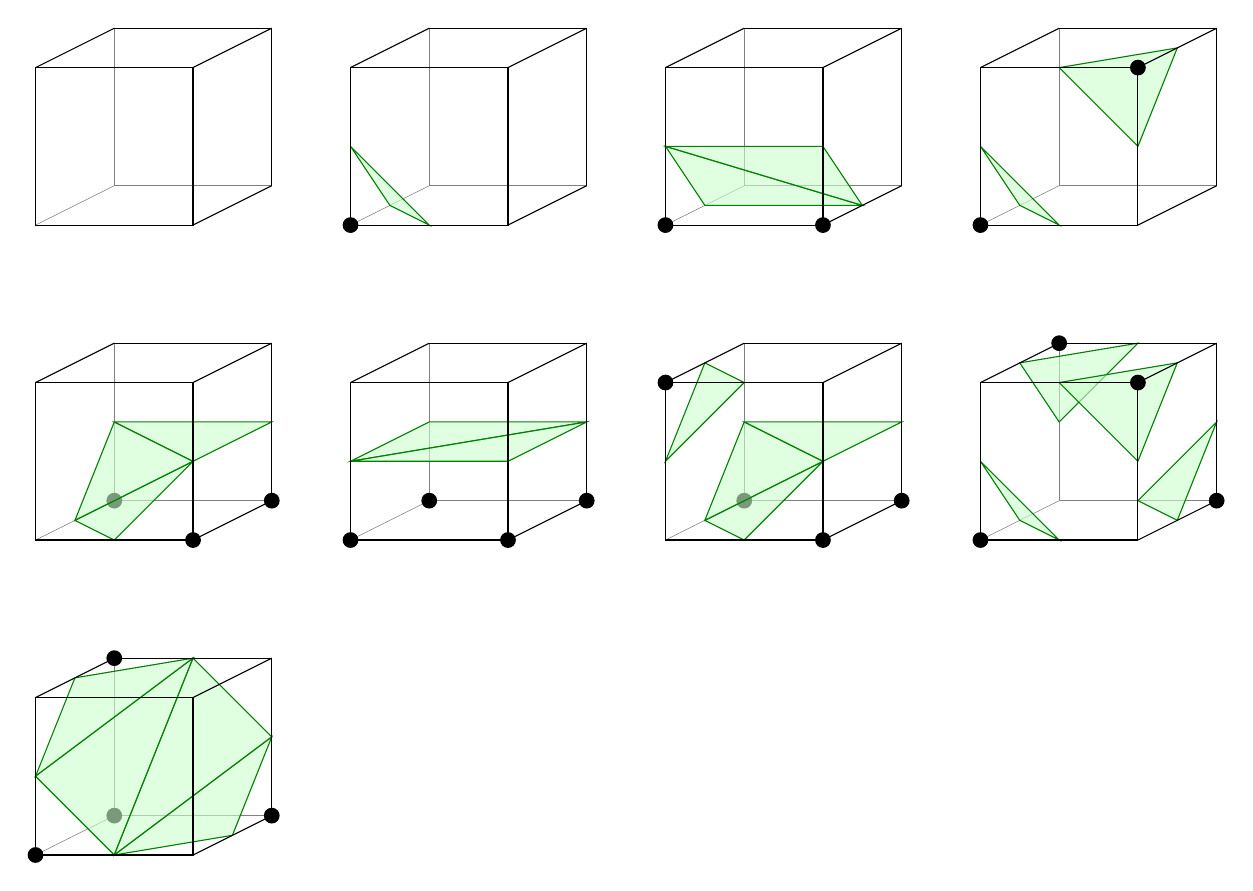
\begin{tikzpicture}[z={(-0.5cm,-0.25cm)}, scale=2]
  \tikzstyle{vertexfill} = [fill=green!20, fill opacity=0.6, draw=green!50!black]

  \def\cubeback{
    \draw[gray,very thin] +(0,0,-1) rectangle +(1,1,-1);
    \draw[gray,very thin] +(0,0,0) -- +(0,0,-1);
  }
  \def\cubefront{
    \draw +(1,0,-1) -- +(1,1,-1);
    \draw +(0,1,-1) -- +(1,1,-1);
    \draw +(0,0,0) rectangle +(1,1,0);
    \draw +(0,1,0) -- +(0,1,-1);
    \draw +(1,0,0) -- +(1,0,-1);
    \draw +(1,1,0) -- +(1,1,-1);
  }

  \begin{scope}[shift={(0,0)}]
    \cubeback
    \cubefront
  \end{scope}

  \begin{scope}[shift={(2,0)}]
    \cubeback
    \filldraw[vertexfill]
      (0,0.5,0) -- (0,0,-0.5) -- (0.5,0,0) -- cycle;
    \fill (0,0) circle (0.05);
    \cubefront
  \end{scope}

  \begin{scope}[shift={(4,0)}]
    \cubeback
    \filldraw[vertexfill]
      (0,0,-0.5) -- (0,0.5,0) -- (1,0,-0.5) -- cycle;
    \filldraw[vertexfill]
      (0,0.5,0) -- (1,0.5,0) -- (1,0,-0.5) -- cycle;
    \fill (0,0) circle (0.05);
    \fill (1,0) circle (0.05);
    \cubefront
  \end{scope}

  \begin{scope}[shift={(6,0)}]
    \cubeback
    \filldraw[vertexfill]
      (0,0.5,0) -- (0,0,-0.5) -- (0.5,0,0) -- cycle;
    \filldraw[vertexfill]
      (1,0.5,0) -- (1,1,-0.5) -- (0.5,1,0) -- cycle;
    \fill (0,0) circle (0.05);
    \fill (1,1) circle (0.05);
    \cubefront
  \end{scope}
  \begin{scope}[shift={(0,-2)}]
    \cubeback
    \fill (0,0,-1) circle (0.05);
    \filldraw[vertexfill]
      (0,0,-0.5) -- (0.5,0,0) -- (1,0.5,0) -- cycle;
    \filldraw[vertexfill]
      (0,0,-0.5) -- (0,0.5,-1) -- (1,0.5,0) -- cycle;
    \filldraw[vertexfill]
      (1,0.5,0) -- (1,0.5,-1) -- (0,0.5,-1) -- cycle;
    
    \fill (1,0) circle (0.05);
    \fill (1,0,-1) circle (0.05);
    \cubefront
  \end{scope}
  \begin{scope}[shift={(2,-2)}]
    \cubeback
    \filldraw[vertexfill]
      (0,0.5,0) -- (1,0.5,-1) -- (0,0.5,-1) -- cycle;
    \filldraw[vertexfill]
      (0,0.5,0) -- (1,0.5,0) -- (1,0.5,-1) -- cycle;

    \fill (0,0) circle (0.05);
    \fill (1,0) circle (0.05);
    \fill (1,0,-1) circle (0.05);
    \fill (0,0,-1) circle (0.05);
    \cubefront
  \end{scope}
  \begin{scope}[shift={(4,-2)}]
    \cubeback
    \fill (0,0,-1) circle (0.05);
    \filldraw[vertexfill]
      (0,0.5,0) -- (0.5,1,0) -- (0,1,-0.5) -- cycle;
    \filldraw[vertexfill]
      (0,0,-0.5) -- (0.5,0,0) -- (1,0.5,0) -- cycle;
    \filldraw[vertexfill]
      (0,0,-0.5) -- (0,0.5,-1) -- (1,0.5,0) -- cycle;
    \filldraw[vertexfill]
      (1,0.5,0) -- (1,0.5,-1) -- (0,0.5,-1) -- cycle;

    \fill (0,1,0) circle (0.05);
    \fill (1,0) circle (0.05);
    \fill (1,0,-1) circle (0.05);
    \cubefront
  \end{scope}
  \begin{scope}[shift={(6,-2)}]
    \cubeback
    \fill (0,1,-1) circle (0.05);
    \fill (1,0,-1) circle (0.05);
    \filldraw[vertexfill]
      (0,1,-0.5) -- (0,0.5,-1) -- (0.5,1,-1) -- cycle;
    \filldraw[vertexfill]
      (0,0.5,0) -- (0,0,-0.5) -- (0.5,0,0) -- cycle;
    \filldraw[vertexfill]
      (1,0.5,0) -- (1,1,-0.5) -- (0.5,1,0) -- cycle;
    \filldraw[vertexfill]
      (1,0,-0.5) -- (1,0.5,-1) -- (0.5,0,-1) -- cycle;

    \fill (1,1) circle (0.05);
    \fill (0,0) circle (0.05);
    \cubefront
  \end{scope}
  \begin{scope}[shift={(0,-4)}]
    \cubeback
    \fill (0,1,-1) circle (0.05);
    \fill (0,0,-1) circle (0.05);
    \fill (1,0,-1) circle (0.05);
    \filldraw[vertexfill]
      (0,0.5,0) -- (0.5,1,-1) -- (0,1,-0.5) -- cycle;
    \filldraw[vertexfill]
      (0,0.5,0) -- (0.5,0,0) -- (0.5,1,-1) -- cycle;
    \filldraw[vertexfill]
      (0.5,0,0) -- (1,0.5,-1) -- (0.5,1,-1) -- cycle;
    \filldraw[vertexfill]
      (0.5,0,0) -- (1,0,-0.5) -- (1,0.5,-1) -- cycle;
    \fill (0,0) circle (0.05);
    \cubefront
  \end{scope}
\end{tikzpicture}

\section{Implementation on GPU with OpenCL}
\subsection{Parallell prefix sum operation}
